% poster template

\documentclass[20pt,margin=1in,innermargin=-4.5in,blockverticalspace=-0.25in]{tikzposter}
\geometry{paperwidth=42in,paperheight=32.5in}
\usepackage[utf8]{inputenc}
\usepackage{amsmath}
\usepackage{amsfonts}
\usepackage{amsthm}
\usepackage{amssymb}
\usepackage{mathrsfs}
\usepackage{graphicx}
\usepackage{adjustbox}
\usepackage{enumitem}
\usepackage[backend=biber,style=numeric]{biblatex}
\usepackage{uomtheme}

\usepackage{mwe} % for placeholder images

\addbibresource{refs.bib}

% set theme parameters
\tikzposterlatexaffectionproofoff
\usetheme{UoMTheme}
\usecolorstyle{UoMStyle}

\usepackage[scaled]{helvet}
\renewcommand\familydefault{\sfdefault} 
\usepackage[T1]{fontenc}

\titlegraphic{\includegraphics[width=0.06\textwidth]{AMTICS.png}}
\title{Semester Hackathon}
\newcommand{\subject}{Deep Learning}
\author{Ayaan Shaikh (202203103510203), Vasanth Sunkara (202203103510405),\\  Vishal Niar (202203103510285), Yaksi Shroff (202203103510201)}
\institute{AMTICS, Uka Tarsadia University}


% begin document
\begin{document}
\maketitle
\centering
\begin{columns}
    \column{0.32}
    \block{Abstract}{
    Leaves play a crucial role in botany and medicine, making accurate classification essential for various applications. This study focuses on the classification of five distinct leaf species—Devil’s Tree, Neem, Desert Rose, Amaranth, and Montessa—using a Convolutional Neural Network (CNN). A deep learning-based approach is employed to efficiently identify and differentiate these species based on image data. The model aims to enhance classification accuracy, contributing to advancements in plant species identification and automated botanical research.
    }
    \block{Introduction}{
   Plants play a vital role in ecology, medicine, and agriculture, making species classification an important task in botany and environmental science. Traditional leaf classification methods rely on manual identification, which can be time-consuming and error-prone. With advancements in artificial intelligence, deep learning techniques, particularly Convolutional Neural Networks (CNNs), have demonstrated remarkable accuracy in image-based classification tasks.

This study focuses on classifying five different leaf species—Devil’s Tree, Neem, Desert Rose, Amaranth, and Montessa—using a CNN model. By leveraging image-based deep learning, the aim is to automate leaf identification with high accuracy, reducing the dependency on manual classification. This research explores the effectiveness of CNNs in plant species recognition.
    }
 \block{Classes}{
 \textbf{1. Neem.}\\
    \begin{tikzfigure}
    \includegraphics[width=0.03\textwidth]{MCLogos/neem/1.jpg}
    \includegraphics[width=0.03\textwidth]{MCLogos/neem/2.jpg}
    \includegraphics[width=0.03\textwidth]{MCLogos/neem/3.jpg}
    \includegraphics[width=0.03\textwidth]{MCLogos/neem/4.jpg}
    \includegraphics[width=0.03\textwidth]{MCLogos/neem/5.jpg}
    \end{tikzfigure} \\

    \textbf{2. Desert Rose Leaf.}\\
    \begin{tikzfigure}
    \includegraphics[width=0.03\textwidth]{MCLogos/rose/1.jpg}
    \includegraphics[width=0.03\textwidth]{MCLogos/rose/2.jpg}
    \includegraphics[width=0.03\textwidth]{MCLogos/rose/3.jpg}
    \includegraphics[width=0.03\textwidth]{MCLogos/rose/4.jpg}
    \includegraphics[width=0.03\textwidth]{MCLogos/rose/5.jpg}
    \end{tikzfigure}

    \textbf{3. Devil's Leaf}.\\
    \begin{tikzfigure}
    \includegraphics[width=0.03\textwidth]{MCLogos/devils/1.jpg}
    \includegraphics[width=0.03\textwidth]{MCLogos/devils/2.jpg}
    \includegraphics[width=0.03\textwidth]{MCLogos/devils/3.jpg}
    \includegraphics[width=0.03\textwidth]{MCLogos/devils/4.jpg}
    \includegraphics[width=0.03\textwidth]{MCLogos/devils/5.jpg}
    \end{tikzfigure}

    \textbf{4. Amarnath.}\\
    \begin{tikzfigure}
    \includegraphics[width=0.03\textwidth]{MCLogos/amarnath/1.jpg}
    \includegraphics[width=0.03\textwidth]{MCLogos/amarnath/2.jpg}
    \includegraphics[width=0.03\textwidth]{MCLogos/amarnath/3.jpg}
    \includegraphics[width=0.03\textwidth]{MCLogos/amarnath/4.jpg}
    \includegraphics[width=0.03\textwidth]{MCLogos/amarnath/5.jpg}
    \end{tikzfigure}

    \textbf{5. Montessa}.\\
    \begin{tikzfigure}
    \includegraphics[width=0.03\textwidth]{MCLogos/montessa/1.jpg}
    \includegraphics[width=0.03\textwidth]{MCLogos/montessa/2.jpg}
    \includegraphics[width=0.03\textwidth]{MCLogos/montessa/3.jpg}
    \includegraphics[width=0.03\textwidth]{MCLogos/montessa/4.jpg}
    \includegraphics[width=0.03\textwidth]{MCLogos/montessa/5.jpg}
    \end{tikzfigure}
    }


    \column{0.36}
    \block{CNN Architecture}{
 
        \begin{tikzfigure}[Architeture.]
            \includegraphics[width=0.9\linewidth]{diagram.png}
        \end{tikzfigure}
        \vspace{2em}


    }
     \block{Trainig Paerformance}{
 
        \begin{tikzfigure}[Training vs Validation Accuracy.]
            \includegraphics[width=0.4\linewidth]{performance_1.jpg}
        \end{tikzfigure}
        \vspace{2em}
        \begin{tikzfigure}[Training vs Validation Loss]
            \includegraphics[width=0.4\linewidth]{performance_2.jpg}
        \end{tikzfigure}

    }

    \column{0.32}
    \block{Result & Model Performance}{
      \textbf{CNN Model Accuracy: 98.80% (Test Set) 
      \\
Loss: 0.0206 (Cross-Entropy)}
\vspace{2em}
\\
  \textbf{Findings : }
       \begin{itemize}
        \item The CNN model effectively differentiates
between leaf species.
        \item Training accuracy improved significantly
after 10 epochs.
        \item Loss decreased steadily, indicating a welloptimized
model.

    \end{itemize}


    }
    
    \block{Conclusion}{
       \textbf{Key Takeaways : }
       \begin{itemize}
        \item The CNN model successfully classified leaf
species with high accuracy
        \item Model performance demonstrates strong
feature extraction capabilities, effectively
distinguishing between Devil’s Tree, Neem,
Desert Rose, Montessa and Amaranth
leaves.
        \item The steady decline in loss and
improvement in accuracy highlight the
model’s robustness.
  \item Future enhancements, such as data
augmentation and hyperparameter tuning,
can further refine accuracy and
generalization.

    \end{itemize}
\\
    }
    
    \block{Future Scope}{
    \\
        This study demonstrates the effectiveness of Convolutional Neural Networks (CNNs) in classifying leaf species with high accuracy. However, several improvements and extensions can be explored in the future:

               \begin{itemize}
   \item \textbf{Expanding the Dataset:} Increasing the number of leaf species and adding more diverse samples, including different lighting conditions and seasonal variations, can enhance model generalization.

     \item \textbf{Improved Model Architecture:} Exploring advanced deep learning models such as Vision Transformers (ViTs) or EfficientNet could further optimize classification accuracy.

 \item \textbf{Real-Time Application:}  Implementing this model in a mobile or web-based application for real-time leaf identification can benefit botanists, farmers, and researchers.

 \item \textbf{Feature Interpretability:} Utilizing explainable AI techniques like Grad-CAM can help visualize which leaf features influence classification decisions.

  \item \textbf{Multimodal Learning:} Combining image-based CNN models with textual botanical descriptions or other plant characteristics can improve classification performance.

    \end{itemize}
    }

    By addressing these aspects, future research can make automated leaf classification more robust, scalable, and applicable to real-world scenarios.
    

\end{columns}
\end{document}